\section{Concept of Smart Home Solution}\label{concept} %28-32 Seiten

	\subsection{Applying measurements}
		The measurements defined in 2.1.4 are applied to Google, Apple and Samsung smart home solutions are compared against each other. SmartThings is a Kickstarter project acquired by Samsung but acting on their own and therefore listed separate. Evaluation is done on a scale from +2 for an excellent compliance to the measurements, all to -1 for not fulfilling the measurements.

		\begin{figure}[h]
			\centering
				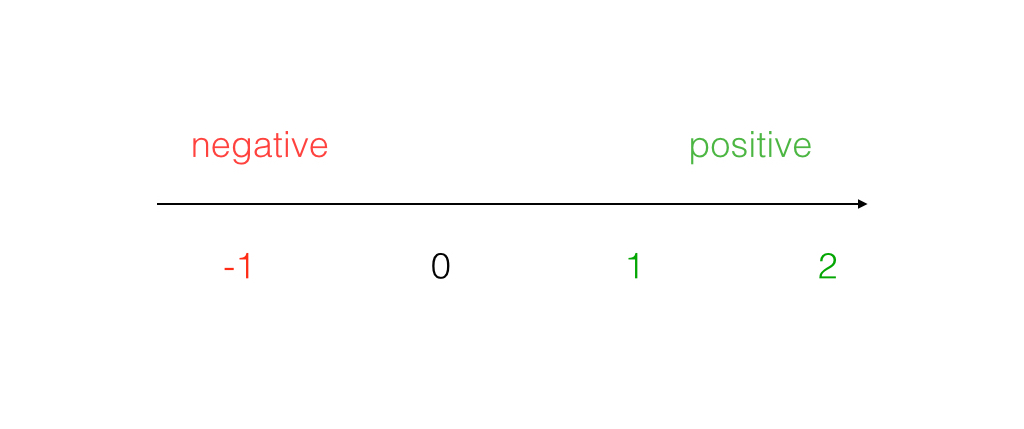
\includegraphics[width=.9\textwidth]{images/praxis/Evaluation.jpg}
			\caption{Evaluation Overview}
			\label{fig:SmartHomeLandscape}
		\end{figure}

		\subsubsection{Some words on trustworthiness}
			Trustworthiness in smart environments is relying on privacy and security. The Ubiquitous Computing Acceptance Model (UCAM) consists of the three mentioned parts and "explains (a) how privacy, security and trust are linked to one another; and (b) how trust is related with usage intention" \parencite{SmartTrust}. Where simple lightbulb controls have nearly no security or privacy impacts, devices like door locks do. The first approach of most iot and smart home novices is to control their light from any device which is regularly not considered to do so. Managing this first hurdle a new wave of home automation is being triggered. Two categories of devices are directly distinguishable:

			\begin{itemize}
				\item sensors
				\item actuators 
			\end{itemize}
			
			Where sensors are used to measure or detect temperature, humidity, daylight or motion, actuators such as motors and switches have a higher risk to do significant damage. 
			%Therefore security is valued high amongst other measurements even though smart home solutions consisting only of sensors are possible.

		\subsubsection{Security}
			\textbf{Apple}
				Apple has reveiled its HomeKit Accessory Protocol (HAP) which is explained in 2.6.3. In summary Apple has invested quite some time in developing a fool proof information transport system between the supported devices. The only downside is that devices need to have more calculation power to provide the HAP security, which leads to lag on non suiting hardware and therefore leads to more expensive devices. Elgato "tweaked the firmware and added additional on-chip memory to handle the heavy-duty encryption" \parencite{HomeKitComputingPower} to suit Apples requirements. Further all device information is stored locally at home.


				\textbf{Apples security system is valued positive (+2).}\\

			\textbf{Google}
				Google claims secure information transportation between devices both locally and through the cloud over Brillos weave. As well as availability for Android and iOS. No further information about technologies were found in the internet \textbf{therefore valued neutral (0).}\\

			\textbf{Samsung}
				Samsung Smart Home solutions dropped 2014 in South Korea and The United States of America \parencite{SamsungComputerBild}. Information on any security systems implemented by Samsung is hardly to find, maybe because there is none. David Lodge, who works for Pen Test Partners has disclosed some major security flaws in Samsungs Smart TVs \parencite{SamsungEncryption}. voice data recorded over the Smart TV is send en clair to third party companies as well as facial recognition information on persons standing in front of the tv \parencite{SamsungEncryption}. 

				\begin{figure}[h]
					\centering
						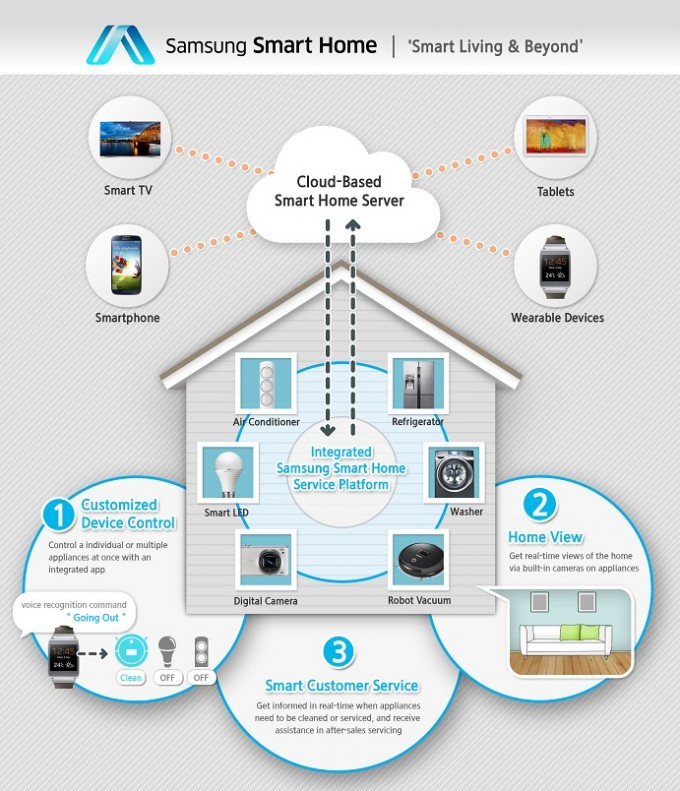
\includegraphics[width=.9\textwidth]{images/theory/samsungSmarthome.jpg}
					\caption{Overview of Samsung Smart Home functionality}
					\label{fig:SmartHomeLandscape}
				\end{figure}

				Considering the fact that Samsungs Smart Home solution is sharing its data over the cloud and no adumbration on any security actions nor on it's official website or elsewhere are made, the educated assumption that there is no special security involved can be made. 

				\textbf{Samsungs security system is valued negative (-1).}\\

			\textbf{SmartThings}
				Lately the SmartThings smart home solution experienced a vulnerability with its cloud communication. Data is in general pushed into the cloud and then send to the according app to notify the user about anything happening at his home. This communication is encrypted using Secure Socket Lacer (SSL) standard. Validation of the cloud servers identity on the hub side is crucial for a secure communication, this is exactly where the failure happened. "This means that an attacker with privileged access to a user’s home network (e.g. physical access) could have executed a “man-in-the-middle” attack that could have decrypted the communications between the SmartThings Hub and the SmartThings Cloud." \parencite{SmartThingsSecurityIssue}. This issue was fixed in a firmware update and further a third party security firm was hired to perform penetration tests on the system. Due to the fact that in general an SSL secured server communication is guaranteed and the security breach was fixed immediately with non affirmed user exploits and the fact that SmartTings will head off the cloud \parencite{SmartThingsCloud}. Further Zigbee and Z-wave are encrypted radios. \textbf{Therefore smartThings is valued positive (+1).}\\
				
			\textbf{Inter-resume}
				With safety in mind Apple is way ahead of other systems like Samsung. Samsung lacking in security is thrown out of the competition at first. SmartThings uses in general secured communication but currently stores all data in the cloud \parencite{SmartThingsCloud}.
	
				\pagebreak

		\subsubsection{Smart home functions}
			\textbf{Apple}
				Apple build up a reliable security standard with the side effects of hardware claiming software. Hence at the time this thesis is written only few manufacturers have fulfilled Apples MFI program and only a handful of devices hit the market. But companies like Insteon are on the right track by providing bridges that connect all of their previously non homekit compatible hardware. Never the less basic functionalities like switches, lightbulbs and environment scanning devices as well as door locks did hit the market, fulfilling six out of seven smart home functions and \textbf{therefore Apple is rated positive (+1).}\\

			\textbf{Google}
				Google covers with it's Nest family consisting of a thermostat, webcam and a smoke sensor relatively small domain of smart home devices compared to Apple, Samsung and SmartThings. Besides the fact that Googles devices comply with five out of seven smart home functions, basic light, switch and door lock compatibilities aren't fulfilled. \textbf{Therefore Google gets a negative credit on smart home functions (-1).}\\

			\textbf{Samsung}
				Samsung is connecting it's smart productline consisting of lightbulbs, vacuum cleaners, refrigerators, washers, door locks and smart tvs all together in it's smart home solution. This quite rich smart home environment complies with six out of seven smart home functions only lacking in indoor environment controlling. \textbf{Therefore a positive rating (+1).}\\

			\textbf{SmartTings}
				SmartThings has a wide variety of smart home devices solving nearly every problem you want to solve with your smart home solution as well as problems that didn't even exist before \textit{feature-ism}. \textbf{Therefore a positive rating (+1).}

				\pagebreak

		\subsubsection{Cross compatibility}
			In this thesis cross compatibility pays special attention to extensibility of systems with third party products. Cross compatibility is valued combining the measurements of the Sullivan rule and future proof ness.\\

			\textbf{Apple}
				In the Apple domain all systems are working like a charm but when it comes to cross compatibility Apple is very poor. Elgato and Insteon  are therefore developing a bridge solution to connect their Smart Home pallet of devices which are inherently not able to speak Cupertino's language \parencite{HomeKitFutureProofness}. Keeping this in mind cross compatibility can be extended to an nearly infinity amount as the bridges are providing connectivity to more proprietary radios like Zigbee and Z-wave. Moreover the \textit{sullivansRule} is fulfilled with the standard HomeKit devices being connected over already existing WiFi or Bluetooth Low Energy. When considering bridges which extend the HomeKit domain extra hardware is necessary, but the benefits overweight the use of one extra hardware:

				"Insteon’s offering makes all of their existing products compatible with HomeKit. This means you can already outfit your entire home, from outlets and plugs to thermostats and locks, with devices that will work with HomeKit. That’s something that not very many companies can offer" \parencite{HomeKitFutureProofness}.

				On the downside currently there is no possibility to connect non Insteon Zigbee or Z-wave solutions \parencite{HomeKitFutureProofness}.

				\textbf{All in all Apple HomeKit is valued positive (+1).}\\

			\textbf{Google}
				Google drives its cross compatibility with the help of its own IoT operation system Brillo, but their considered system nest, consisting only of a thermostat, a smoke sensor and a webcam is not sufficient enough for overall smart home purposes nor fulfilling the smart home functions defined earlier nor in any way cross compatible, \textbf{therefore considered negative (-1).}\\

			\textbf{Samsung}
				Samsung has introduced its Smart Home Protocol (SHP) to enable the communication between different home appliances. Further it is intended to enable third party manufacturer to control their devices over the Samsung cloud. Future plans include Home-Energy, Secure Home Access, Healthcare und Eco Home Applications enabled \parencite{SHP}. Due to the fact that no third party vendors were announced for over a year since Samsung dropped their Smart Home initiative the ability of cross compatibility is valued less than already available products. Current Samsung smart home solutions are 

				\textbf{Samsung is valued negative (-1).}\\

			\textbf{SmartThings}
				SmartTings was developed with wide range compatibility in mind. "Its open system works with a wider selection of gadgets, and developers keep adding compatibility to more devices on a regular basis" \parencite{SmartThingsCompat}. The wide variety of SmartTings compatible devices which can be connected to the hub are in parts useless for the daily life and fall into the category of \textit{feature-ism} therefore being valued negative. Devices always have to be connected to a hub which doesn't serve the measurement of minimalism, but to keep in mind they are cross compatible to many devices and therefore valued positive. \textbf{All in all cross compatibility is valued positive (+2).}\\

			\textbf{Inter-resume}
				Further a distinction must be made between smart home solutions like Apple which only provide software in form of services and protocols for third party companies which then have to implement Apples standards in order to play their part, where Samsung and Google provide their own hardware. SmartThings on the other hand provides software in form of an app as well as a dedicated hub which allows third party systems to connect to. At the time this thesis is written, only Apple and SmartThings provide the ability to connect devices that are not specifically intended to work with the system. Moreover of the two just Apple HomeKit is out of the box voice controlled. Further more "mature" vendors like Elgato and Insteon provide a hub which provide connectivity of their none HomeKit product line to control them over the Apple solution. Google with its thin product line loses the cross compatibility race and its non-compliance in the predefined smart home functions.

				\textbf{intermediate result}
					\begin{itemize}
						\item Apple 		+4
						\item Google		-2
						\item Samsung 		-1
						\item SmartThings 	+4
					\end{itemize}


				%\pagebreak

		\subsubsection{Cost}
			%and futureproofness
			All of the compared systems require smart phones in order to send commands and read out sensor data from smart home devices. For the cost calculation these smart phones will not be added to the total costs. It is questionable whether or not smart watches should be considered for the total cost estimation. Due to the fact that they are not required to operate a smart home and just have a subset of functions compared to there big brother phones they are not considered in the computation of costs. 

			\textbf{Apple}
				Apple certified smart devices are in the range of 50 to 200 Dollar. (1)\\

			\textbf{Google}
				Nest device costs are in the range of 99 to 200 Dollar.(1)\\

			\textbf{Samsung}
				Samsung smart home solutions are pretty cost intensive because their line of devices are regular domestic appliances with a little logic in it to communicate to an app. Therefore cost ranges start at 150 up to multiple thousand Dollars.(0)\\

			\textbf{SmartThings}
				A smarttings hub costs 100 Dollar.(1)
			
			%\pagebreak

		\subsubsection{Extra}
			Extra points for minimalism are assigned if the smart home solution is providing voice control.

			\textbf{Apple}
				Apple provides out of the box voice control with the help of its spaech assistant siri \parencite{IntroToHomeKit}. this is a big step into seamless smart home controlling and fulfilling the minimalism criteria. Therefore an extra point for Apple (+1).\\

			\textbf{Google}
				Google as well provides voice control functionality and gets an extra point (+1).\\

			\textbf{Samsung}\\
				Samsung as well provides voice control functionality and gets an extra point (+1).\\

			\textbf{SmartTings}
				SmartThings is natively not supporting voice control, therefore zero extra points (0).\\

			\pagebreak

		\subsubsection{Comparison}

			The points total are shown in the following table:

			\begin{table}[h]
				\centering
				\caption{Evaluation of smart home solutions}
				\label{Homekit_Accessory_Profile}
				\begin{tabular}{lllll}
					\textbf{Services}		& \textbf{Apple} 	& \textbf{Google}	& \textbf{Samsung}	& \textbf{SmartThings}	\\
					\hline
					Security				& 2					& 0 				& -1				& 1 \\
					Smart Home Functions	& 1					& -1 				& 1 				& 1	\\
					Cross Compatibility		& 1					& -1 				& -1				& 2	\\
					Costs					& 1					& 1					& 0					& 1 \\
					Extra					& 1 				& 1					& 1					& 0 \\
					\hline
					Overall					& 6					& 0					& 0 				& 5 \\
				\end{tabular}
			\end{table}


		\subsubsection{The winner}
				Apple wins the competition hence the solution will be build upon HomeKit.

		\pagebreak

	\subsection{Concept} 
		The basic idea of connecting SDPvNext and Apple HomeKit is to write a middleware which is running on a homeg ateway and providing a connection to SDPvNext as well as pushing the devices with HomeKit meta data into the local network in order to control them over iDevices and Siri. For clarification purposes a graphic of the idea is given:


		\begin{figure}[h]
				\centering
					\includegraphics[width=.9\textwidth]{images/praxis/ConceptIdea.jpg}
				\caption{Concept idea}
				\label{fig:ConceptIdea}
		\end{figure}

		\pagebreak

		\subsubsection{Possible solutions}
			Revisiting the graphic of HomeKits functionality, there are two possible solutions for an interconnectivity to SDPvNext marked in blue:

			\begin{figure}[h]
				\centering
					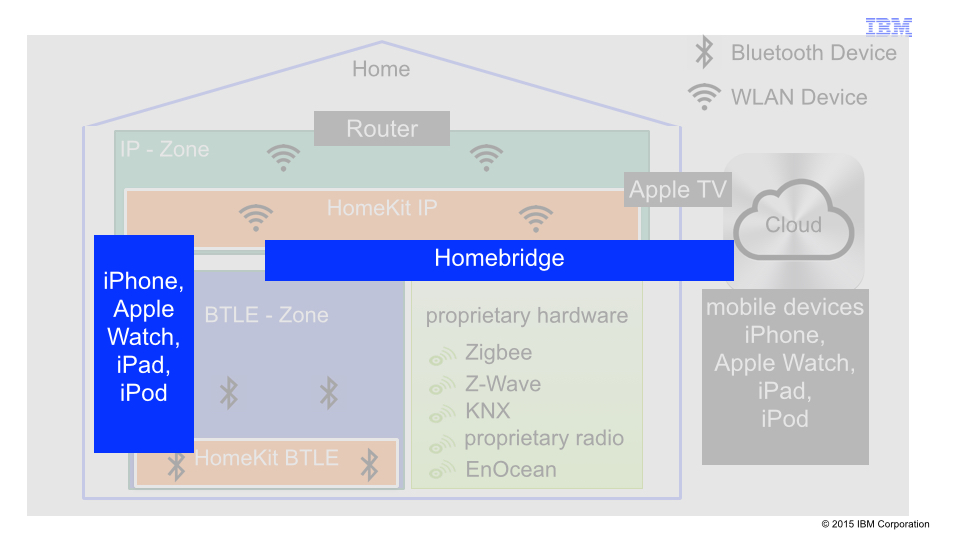
\includegraphics[width=.9\textwidth]{images/praxis/MiddlewarePossibilities.jpg}
				\caption{HomeKit middleware possibilities}
				\label{fig:SmartHomeLandscape}
			\end{figure} 

			On one hand a bridge equipped with extra software providing non HomeKit, SDPvNext provided devices the ability to be managed by Apple. On the other hand an iOS app using the SDPvNext rest and HomeKit api to provide inter connect ability between the two smart home solutions.

			\pagebreak

			\textbf{Bridge solution}
				The bridge solution would aggregate non HomeKit devices connected to a homeg ateway in order to present them as HomeKit compatible devices in a WiFi environment.

				\begin{figure}[h]
					\centering
						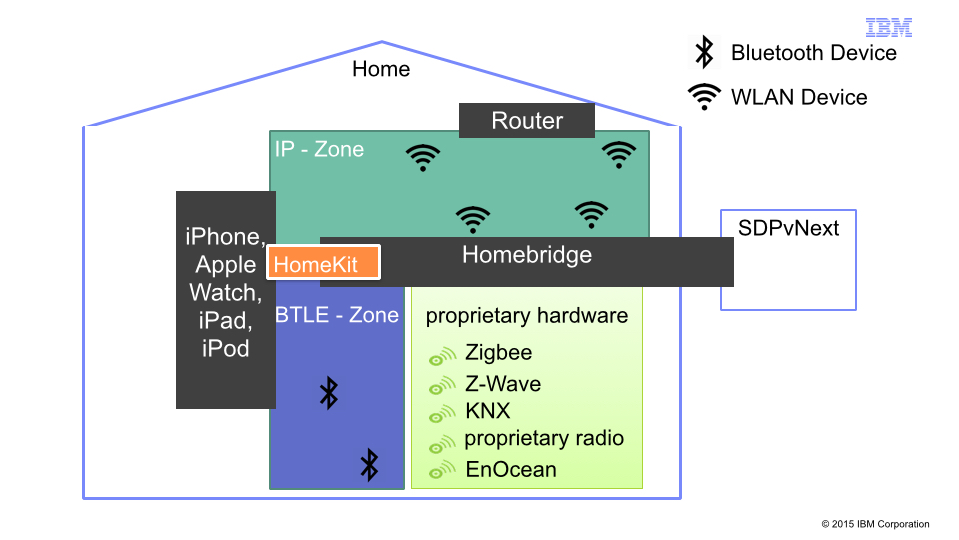
\includegraphics[width=.9\textwidth]{images/praxis/BridgeSolution.jpg}
					\caption{Overview BridgeSolution}
					\label{fig:SmartHomeLandscape}
				\end{figure} 	

			\textbf{SDPvNext Rest API + iOS App}
				The iOS App makes use of the SDPvNext Rest Api to get information about connected devices and stores them in the HomeKit database.

				\begin{figure}[h]
					\centering
						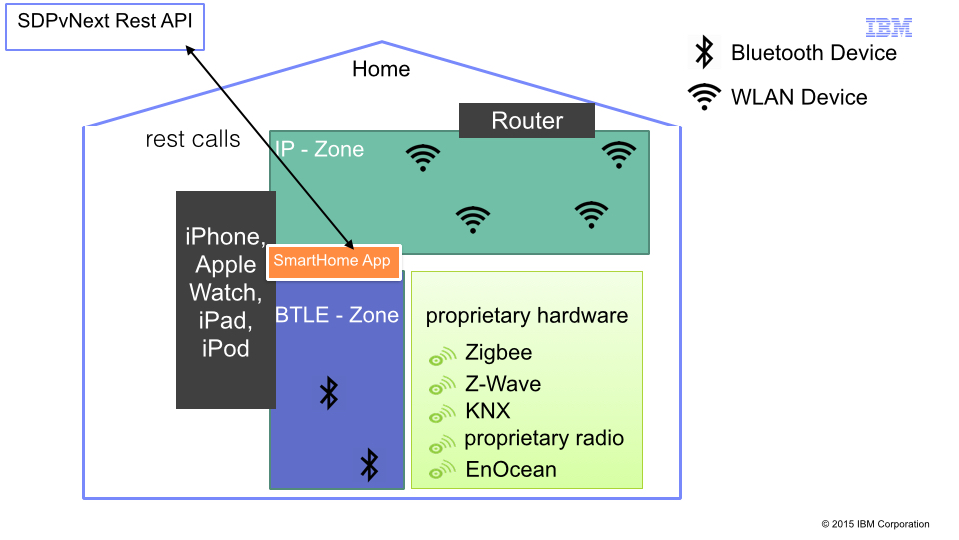
\includegraphics[width=.9\textwidth]{images/praxis/iOSSolution.jpg}
					\caption{Overview iOS Solution}
					\label{fig:SmartHomeLandscape}
				\end{figure} 	

				\pagebreak

		\subsubsection{Advantages and disadvantages}
			\textbf{Bridge solution}
				The advantages and disadvantages of the bridge solution are provided in the following table:

				\begin{table}[h]
					\centering
					\caption{Advantages and disadvantages of the bridge solution}
					\label{Homekit_Accessory_Profile}
					\begin{tabular}{p{5cm}p{5cm}}
						\textbf{Advantages}		& \textbf{Disadvantages} \\
						\hline
						Proprietary radios can be connected directly to the home gateway without the workaround of SDPvNext.		& The bridge solution requires extra hardware in terms of a home gateway that provides server functions in order to represent non HomeKit hardware. \\
											& Access to the Apple MFI program in necessary in order to be able to officially use the HAP protocol and therefore the bridge solution\\
					\end{tabular}
				\end{table}
				

			\textbf{SDPvNext Rest API + iOS App}
				\begin{table}[h]
					\centering
					\caption{Advantages and disadvantages of the iOS solution}
					\label{Homekit_Accessory_Profile}
					\begin{tabular}{p{5cm}p{5cm}}
						\textbf{Advantages}		& \textbf{Disadvantages} \\
						\hline
						The iOS App solution is independent of extra hardware		& The iOS solution has to implement the HomeKit api and extra logic has to be added to the SDPvNext environment to cover meta data necessary to operate the HomeKit database. \\
					\end{tabular}
				\end{table}

				\pagebreak
				

		%\subsubsection{Use Cases covered}

		%\subsubsection{Measurements}
			%The measurements defined in 2.1.4 are applied to the solution in order to value the outcome.\\

			%\textbf{Reliability of Manufactors}
				% #longterminvestment

			%\textbf{Security}
				%Stromausfall -> BTLE
				%Datenaustausch

			%\textbf{cross compatibility}

			%\textbf{setup}

			%\pagebreak

	\subsection{Solution} 
		The middleware's task is to connect to SDPvNext, load a json configuration file with all the information about the connected devices and store them into the HomeKit database. Further implementation includes enabling an http post request to set device states and to allow interaction. Apple provides a sample app where the whole spectrum of the HomeKit api is implemented \parencite{AppleHomeKitSample}. This sample code can be accessed by anyone that registers to Apples developer program. To not exceed the frame of this thesis the sample code is not explained. Further the iOS solution explanation will not cover how devices will be connected to HomeKit and written to the database. There is plenty documentation in the web that explains how this is done. Lastly a WatchKit interface with a shared datastore is covered in order to view and manage your devices from the Apple Watch. \\

		\subsubsection{Design}
			The iOS app has four core functions that have to be implemented in order to show devices from SDPvNext.
			
		\pagebreak
		\subsubsection{Implementation} 

			To keep the implementation simple the solution will be divided into five milestones:

			\begin{itemize}
				\item SDPvNext rest api
				\item Json parsing
				\item Presentation
				\item Apple WatchKit
				\item Data exchange
			\end{itemize}

			\textbf{SDPvNext rest api}
				First of all a connection has to be build up to the SDPvNext rest api. In order to accomplish this minor tasks have to be fulfilled. 


				The header for the connection has to be filled with authentication and request method information:

				\begin{lstlisting}[caption=Authentication Setup] 
	    		let username = "userName"
	    		let password = "password"
	    		let loginString = NSString(format: "%@:%@", username, password)
	    		let loginData: NSData = loginString.dataUsingEncoding(NSUTF8StringEncoding)!
	    		let base64LoginString = loginData.base64EncodedStringWithOptions(nil) 
				\end{lstlisting} 

				Credentials have to be base64 encoded.

				\begin{lstlisting}[caption=Request Setup] 
				var Error: NSError?
	        	var Url: NSURL = NSURL(string: "here comes the url")!
	        	let Request = NSMutableURLRequest(URL: Url)
	        	Request.HTTPMethod = "GET"
	        	Request.setValue("Basic \(base64LoginString)", forHTTPHeaderField: "Authorization")
	        	var Response: NSURLResponse?
				\end{lstlisting}

				Further the connection is started and received data is stored.

				\begin{lstlisting}[caption=Create connection to receive json]
				var Data = NSURLConnection.sendSynchronousRequest(Request, returningResponse: &Response, error: &Error) as NSData?
	        	\end{lstlisting}

	        	\pagebreak

			\textbf{Json parsing}
				For further procedures the status code is checked whether or not the request was successfull.

	        	\begin{lstlisting}[caption=Check whether request was successfull]
	        	if let httpResponse = Response as? NSHTTPURLResponse {
	            	if(httpResponse.statusCode == 200){
	                	let parsedObject: AnyObject? = NSJSONSerialization.JSONObjectWithData(Data!, options: NSJSONReadingOptions.AllowFragments, error:nil)
	                		...
	        	\end{lstlisting}

	        	Json data is parsed into an NSDictionary to get access to the inquired values. A dummy object is created to store the values.

	        	\begin{lstlisting}[caption=Json parsing]
	        	...
	        	if let json = parsedObject as? NSDictionary {
	                    for (key, value) in json{
	                        if key as! String == "children"{
	                            let children = value as! NSArray
	                            for child in children{
	                                var device = [
	                                    "no_location",
	                                    "no_tenant",
	                                    "no_name",
	                                    "no_href",
	                                    "no_type",
	                                    "no_switch"
	                                ]
	                             	...
	        	\end{lstlisting}

	        	This is an example of how iteration through the different children is done.

	        	\begin{lstlisting}[caption=Json iteration]
	        	...
	        	if let location = child["location"] as? NSString{
	                                    device[0] = location as String
	                                }
	                             	...
	        	\end{lstlisting}

	        \pagebreak

	        \textbf{Send change requests}
				SDPvNext in its current stage is not able to process any interaction over the rest api, however to make the middleware interactive a shaspa bridge rest api is used to send json in order to control connected devices.
				Where the connecting part is the same, the type of request has to be POST. Further a json string has to be build:

				\begin{lstlisting}[caption=Json build]
	        	let jsonString = "{\"obix\":\"obj\",\"name\":\"\("e.g. the name")\",\"tenant\":\"\("e.g the user")\",\"children\":[{\"obix\":\"bool\",\"name\":\"Status\",\"val\":\"\("e.g. the status which is set (e.g. either on or off)")\"}]}"
	        	\end{lstlisting}

	        	In addition the header information has to be updated to consist \textit{application/json} data:

	        	\begin{lstlisting}[caption=Additional header information]
	        	Request.HTTPBody = jsonString.dataUsingEncoding(NSUTF8StringEncoding, allowLossyConversion: false)
        		Request.setValue("application/json", forHTTPHeaderField: "Content-Type")
	        	\end{lstlisting}

	        	\pagebreak

			\textbf{Presentation}
				Devices will be presented in a table view with a foldout submenu featuring an on/off button as well as a status label. This label houses many different values ranging from temperature to operating states:

				\begin{figure}[h]
					\centering
						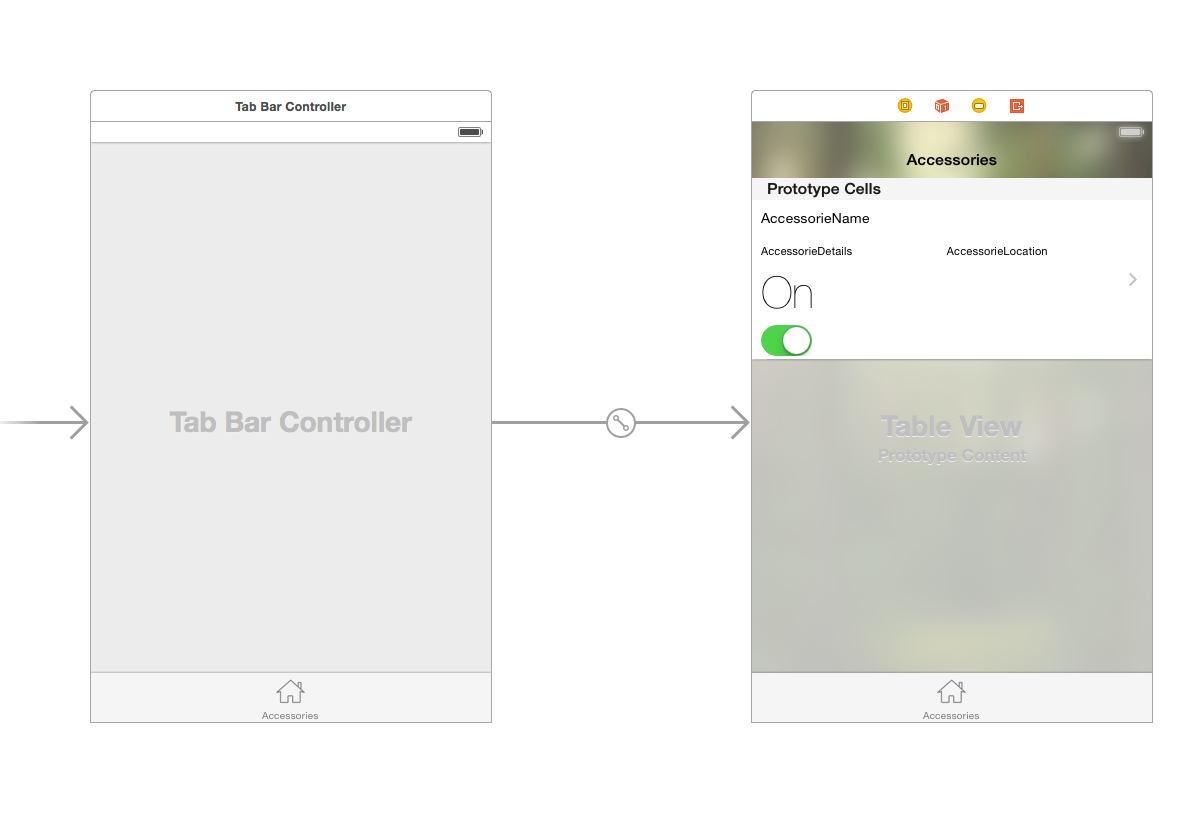
\includegraphics[width=.9\textwidth]{images/praxis/SmartHomeAppDesignOverview.png}
					\caption{Device presentation}
					\label{fig:ConceptIdea}
				\end{figure}

			\textbf{Apple WatchKit}
				The interface running on the Apple Watch looks somewhat similar to the iOS app. Only difference is that the app is only displaying a filtered list of devices that can be managed directly, not including devices like servers or home gateways. This is necessary because of the small form factor of the watch's display. In addition to the iOS app property information is realized by a segue to a new detail view.

				\begin{figure}[h]
					\centering
						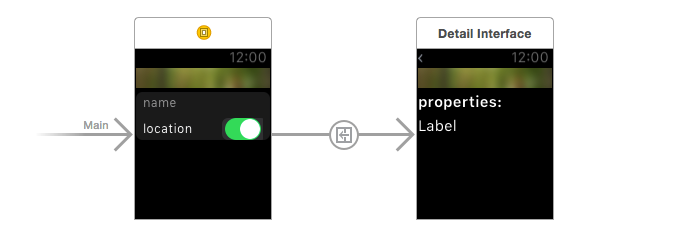
\includegraphics[width=.9\textwidth]{images/praxis/SmartHomeWatchkitInterface.png}
					\caption{Watchkit interface}
					\label{fig:ConceptIdea}
				\end{figure}

	        	\pagebreak

			\textbf{Data exchange}

				Exchange of data is handled by a datastore between the iOS and WatchKit app. This feature has to be enabled in the iOS apps capabilities. The DatastoreProtocol stores the keys that are used to identify the values in the datastore.

				\begin{lstlisting}[caption=DataStore keys]
				let kaccessorieName     = "kaccessorieName"
				let kaccessorieType     = "kaccessorieType"
				let kaccessorieLoc      = "kaccessorieLoc"
				let kaccessorieProp     = "kaccessorieProp"
				let kaccessorieStat     = "kaccessorieStat"
				let kaccessorieHref     = "kaccessorieHref"
				let kaccessorieTenant   = "kaccessorieTenant"

				protocol DatastoreProtocol {
				    func save(#key: String, value: NSArray)
				    func load<T>(#key: String) -> T?
				    func commitToDisk()
				}
	        	\end{lstlisting}

	        	The default datastore has to be specified as well as the type of data that is stored. Additionally methods to write and load from the datastore are provided.

	        	\begin{lstlisting}[caption= Custom dataStore]
	        	//created custom dataStore: "here comes your datastore"
				class SharedUserDefaultsDatastore: NSObject, DatastoreProtocol {
				    let userDefaults = NSUserDefaults(suiteName: "datastore url")!
				    
				    func save(#key: String, value: NSArray) {
				        userDefaults.setObject(value, forKey: key)
				    }
				    
				    func load<T>(#key: String) -> T? {
				        let obj: AnyObject? = userDefaults.objectForKey(key)
				        
				        if let validObj = obj as? T {
				            return validObj
				        }
				        else {
				            return nil
				        }
				    }
				    
				    func commitToDisk() {
				        userDefaults.synchronize()
				    }
				}
	        	\end{lstlisting}

				\pagebreak

		%\subsubsection{Test}

			%\pagebreak

		\subsubsection{Additional work}
			The given implementation shows how devices can be loaded from SDPvNext and how the received json is parsed to access information. As already mentioned the HomeKit api is not explicitly covered due to the fact that this topic would fill an entire thesis on its own. This does not imply that further research on this theme is obsolete. To add devices to the HomeKit database additional meta data is required as well as a pairing code for every single device.


			\textbf{Problem}
				The SDPvNext's backend has to store these additional information to provide full cross compatibility coverage. Changes in the backend of SDPvNext are out of the scope of this thesis but will be recommend to the developers. At least the possibility to load simple prototypes that match all the necessary requirements for a HomeKit device should be implemented to enable a cross compatibility of 100\%.

\pagebreak